\documentclass[1p]{elsarticle_modified}
%\bibliographystyle{elsarticle-num}

%\usepackage[colorlinks]{hyperref}
%\usepackage{abbrmath_seonhwa} %\Abb, \Ascr, \Acal ,\Abf, \Afrak
\usepackage{amsfonts}
\usepackage{amssymb}
\usepackage{amsmath}
\usepackage{amsthm}
\usepackage{scalefnt}
\usepackage{amsbsy}
\usepackage{kotex}
\usepackage{caption}
\usepackage{subfig}
\usepackage{color}
\usepackage{graphicx}
\usepackage{xcolor} %% white, black, red, green, blue, cyan, magenta, yellow
\usepackage{float}
\usepackage{setspace}
\usepackage{hyperref}

\usepackage{tikz}
\usetikzlibrary{arrows}

\usepackage{multirow}
\usepackage{array} % fixed length table
\usepackage{hhline}

%%%%%%%%%%%%%%%%%%%%%
\makeatletter
\renewcommand*\env@matrix[1][\arraystretch]{%
	\edef\arraystretch{#1}%
	\hskip -\arraycolsep
	\let\@ifnextchar\new@ifnextchar
	\array{*\c@MaxMatrixCols c}}
\makeatother %https://tex.stackexchange.com/questions/14071/how-can-i-increase-the-line-spacing-in-a-matrix
%%%%%%%%%%%%%%%

\usepackage[normalem]{ulem}

\newcommand{\msout}[1]{\ifmmode\text{\sout{\ensuremath{#1}}}\else\sout{#1}\fi}
%SOURCE: \msout is \stkout macro in https://tex.stackexchange.com/questions/20609/strikeout-in-math-mode

\newcommand{\cancel}[1]{
	\ifmmode
	{\color{red}\msout{#1}}
	\else
	{\color{red}\sout{#1}}
	\fi
}

\newcommand{\add}[1]{
	{\color{blue}\uwave{#1}}
}

\newcommand{\replace}[2]{
	\ifmmode
	{\color{red}\msout{#1}}{\color{blue}\uwave{#2}}
	\else
	{\color{red}\sout{#1}}{\color{blue}\uwave{#2}}
	\fi
}

\newcommand{\Sol}{\mathcal{S}} %segment
\newcommand{\D}{D} %diagram
\newcommand{\A}{\mathcal{A}} %arc


%%%%%%%%%%%%%%%%%%%%%%%%%%%%%5 test

\def\sl{\operatorname{\textup{SL}}(2,\Cbb)}
\def\psl{\operatorname{\textup{PSL}}(2,\Cbb)}
\def\quan{\mkern 1mu \triangleright \mkern 1mu}

\theoremstyle{definition}
\newtheorem{thm}{Theorem}[section]
\newtheorem{prop}[thm]{Proposition}
\newtheorem{lem}[thm]{Lemma}
\newtheorem{ques}[thm]{Question}
\newtheorem{cor}[thm]{Corollary}
\newtheorem{defn}[thm]{Definition}
\newtheorem{exam}[thm]{Example}
\newtheorem{rmk}[thm]{Remark}
\newtheorem{alg}[thm]{Algorithm}

\newcommand{\I}{\sqrt{-1}}
\begin{document}

%\begin{frontmatter}
%
%\title{Boundary parabolic representations of knots up to 8 crossings}
%
%%% Group authors per affiliation:
%\author{Yunhi Cho} 
%\address{Department of Mathematics, University of Seoul, Seoul, Korea}
%\ead{yhcho@uos.ac.kr}
%
%
%\author{Seonhwa Kim} %\fnref{s_kim}}
%\address{Center for Geometry and Physics, Institute for Basic Science, Pohang, 37673, Korea}
%\ead{ryeona17@ibs.re.kr}
%
%\author{Hyuk Kim}
%\address{Department of Mathematical Sciences, Seoul National University, Seoul 08826, Korea}
%\ead{hyukkim@snu.ac.kr}
%
%\author{Seokbeom Yoon}
%\address{Department of Mathematical Sciences, Seoul National University, Seoul, 08826,  Korea}
%\ead{sbyoon15@snu.ac.kr}
%
%\begin{abstract}
%We find all boundary parabolic representation of knots up to 8 crossings.
%
%\end{abstract}
%\begin{keyword}
%    \MSC[2010] 57M25 
%\end{keyword}
%
%\end{frontmatter}

%\linenumbers
%\tableofcontents
%
\newcommand\colored[1]{\textcolor{white}{\rule[-0.35ex]{0.8em}{1.4ex}}\kern-0.8em\color{red} #1}%
%\newcommand\colored[1]{\textcolor{white}{ #1}\kern-2.17ex	\textcolor{white}{ #1}\kern-1.81ex	\textcolor{white}{ #1}\kern-2.15ex\color{red}#1	}

{\Large $\underline{12n_{0566}~(K12n_{0566})}$}

\setlength{\tabcolsep}{10pt}
\renewcommand{\arraystretch}{1.6}
\vspace{1cm}\begin{tabular}{m{100pt}>{\centering\arraybackslash}m{274pt}}
\multirow{5}{120pt}{
	\centering
	\includegraphics[width=112pt]{../../../GIT/diagram.site/Diagrams/png/2655_12n_0566.png}\\
\ \ \ A knot diagram\footnotemark}&
\allowdisplaybreaks
\textbf{Linearized knot diagam} \\
\cline{2-2}
 &
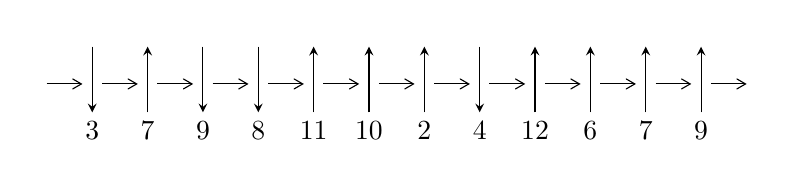
\begin{tikzpicture}[x=20pt, y=17pt]
	% nodes
	\node (C0) at (0, 0) {};
	\node (C1) at (1, 0) {};
	\node (C1U) at (1, +1) {};
	\node (C1D) at (1, -1) {3};

	\node (C2) at (2, 0) {};
	\node (C2U) at (2, +1) {};
	\node (C2D) at (2, -1) {7};

	\node (C3) at (3, 0) {};
	\node (C3U) at (3, +1) {};
	\node (C3D) at (3, -1) {9};

	\node (C4) at (4, 0) {};
	\node (C4U) at (4, +1) {};
	\node (C4D) at (4, -1) {8};

	\node (C5) at (5, 0) {};
	\node (C5U) at (5, +1) {};
	\node (C5D) at (5, -1) {11};

	\node (C6) at (6, 0) {};
	\node (C6U) at (6, +1) {};
	\node (C6D) at (6, -1) {10};

	\node (C7) at (7, 0) {};
	\node (C7U) at (7, +1) {};
	\node (C7D) at (7, -1) {2};

	\node (C8) at (8, 0) {};
	\node (C8U) at (8, +1) {};
	\node (C8D) at (8, -1) {4};

	\node (C9) at (9, 0) {};
	\node (C9U) at (9, +1) {};
	\node (C9D) at (9, -1) {12};

	\node (C10) at (10, 0) {};
	\node (C10U) at (10, +1) {};
	\node (C10D) at (10, -1) {6};

	\node (C11) at (11, 0) {};
	\node (C11U) at (11, +1) {};
	\node (C11D) at (11, -1) {7};

	\node (C12) at (12, 0) {};
	\node (C12U) at (12, +1) {};
	\node (C12D) at (12, -1) {9};
	\node (C13) at (13, 0) {};

	% arrows
	\draw[->,>={angle 60}]
	(C0) edge (C1) (C1) edge (C2) (C2) edge (C3) (C3) edge (C4) (C4) edge (C5) (C5) edge (C6) (C6) edge (C7) (C7) edge (C8) (C8) edge (C9) (C9) edge (C10) (C10) edge (C11) (C11) edge (C12) (C12) edge (C13) ;	\draw[->,>=stealth]
	(C1U) edge (C1D) (C2D) edge (C2U) (C3U) edge (C3D) (C4U) edge (C4D) (C5D) edge (C5U) (C6D) edge (C6U) (C7D) edge (C7U) (C8U) edge (C8D) (C9D) edge (C9U) (C10D) edge (C10U) (C11D) edge (C11U) (C12D) edge (C12U) ;
	\end{tikzpicture} \\
\hhline{~~} \\& 
\textbf{Solving Sequence} \\ \cline{2-2} 
 &
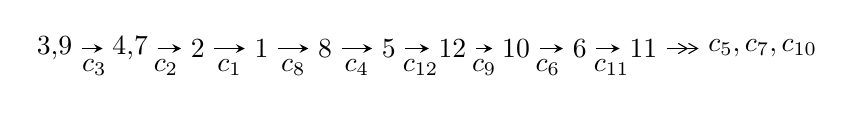
\begin{tikzpicture}[x=23pt, y=7pt]
	% node
	\node (A0) at (-1/8, 0) {3,9};
	\node (A1) at (17/16, 0) {4,7};
	\node (A2) at (17/8, 0) {2};
	\node (A3) at (25/8, 0) {1};
	\node (A4) at (33/8, 0) {8};
	\node (A5) at (41/8, 0) {5};
	\node (A6) at (49/8, 0) {12};
	\node (A7) at (57/8, 0) {10};
	\node (A8) at (65/8, 0) {6};
	\node (A9) at (73/8, 0) {11};
	\node (C1) at (1/2, -1) {$c_{3}$};
	\node (C2) at (13/8, -1) {$c_{2}$};
	\node (C3) at (21/8, -1) {$c_{1}$};
	\node (C4) at (29/8, -1) {$c_{8}$};
	\node (C5) at (37/8, -1) {$c_{4}$};
	\node (C6) at (45/8, -1) {$c_{12}$};
	\node (C7) at (53/8, -1) {$c_{9}$};
	\node (C8) at (61/8, -1) {$c_{6}$};
	\node (C9) at (69/8, -1) {$c_{11}$};
	\node (A10) at (11, 0) {$c_{5},c_{7},c_{10}$};

	% edge
	\draw[->,>=stealth]	
	(A0) edge (A1) (A1) edge (A2) (A2) edge (A3) (A3) edge (A4) (A4) edge (A5) (A5) edge (A6) (A6) edge (A7) (A7) edge (A8) (A8) edge (A9) ;
	\draw[->>,>={angle 60}]	
	(A9) edge (A10);
\end{tikzpicture} \\ 

\end{tabular} \\

\footnotetext{
The image of knot diagram is generated by the software ``\textbf{Draw programme}" developed by Andrew Bartholomew(\url{http://www.layer8.co.uk/maths/draw/index.htm\#Running-draw}), where we modified some parts for our purpose(\url{https://github.com/CATsTAILs/LinksPainter}).
}\phantom \\ \newline 
\centering \textbf{Ideals for irreducible components\footnotemark of $X_{\text{par}}$} 
 
\begin{align*}
I^u_{1}&=\langle 
-4.65742\times10^{21} u^{31}-2.20023\times10^{22} u^{30}+\cdots+9.36708\times10^{23} b+5.12230\times10^{23},\\
\phantom{I^u_{1}}&\phantom{= \langle  }2.94856\times10^{25} u^{31}-3.10386\times10^{25} u^{30}+\cdots+2.99747\times10^{25} a-2.87196\times10^{25},\;u^{32}- u^{31}+\cdots-2 u+1\rangle \\
I^u_{2}&=\langle 
b- u,\;a^5- a^4+2 a^3- a^2+a-1,\;u^2+1\rangle \\
I^u_{3}&=\langle 
b- u,\;a,\;u^6- u^5+2 u^4-2 u^3+2 u^2-2 u+1\rangle \\
I^u_{4}&=\langle 
b- u,\;a,\;u^3+u^2+2 u+1\rangle \\
\\
\end{align*}
\raggedright * 4 irreducible components of $\dim_{\mathbb{C}}=0$, with total 51 representations.\\
\footnotetext{All coefficients of polynomials are rational numbers. But the coefficients are sometimes approximated in decimal forms when there is not enough margin.}
\newpage
\renewcommand{\arraystretch}{1}
\centering \section*{I. $I^u_{1}= \langle -4.66\times10^{21} u^{31}-2.20\times10^{22} u^{30}+\cdots+9.37\times10^{23} b+5.12\times10^{23},\;2.95\times10^{25} u^{31}-3.10\times10^{25} u^{30}+\cdots+3.00\times10^{25} a-2.87\times10^{25},\;u^{32}- u^{31}+\cdots-2 u+1 \rangle$}
\flushleft \textbf{(i) Arc colorings}\\
\begin{tabular}{m{7pt} m{180pt} m{7pt} m{180pt} }
\flushright $a_{3}=$&$\begin{pmatrix}1\\0\end{pmatrix}$ \\
\flushright $a_{9}=$&$\begin{pmatrix}0\\u\end{pmatrix}$ \\
\flushright $a_{4}=$&$\begin{pmatrix}1\\u^2\end{pmatrix}$ \\
\flushright $a_{7}=$&$\begin{pmatrix}-0.983683 u^{31}+1.03549 u^{30}+\cdots+42.1633 u+0.958130\\0.00497211 u^{31}+0.0234890 u^{30}+\cdots+1.12532 u-0.546841\end{pmatrix}$ \\
\flushright $a_{2}=$&$\begin{pmatrix}0.495029 u^{31}-0.483684 u^{30}+\cdots+26.1222 u-0.952046\\-0.0284611 u^{31}+0.0288036 u^{30}+\cdots+0.536896 u-0.995028\end{pmatrix}$ \\
\flushright $a_{1}=$&$\begin{pmatrix}0.466568 u^{31}-0.454881 u^{30}+\cdots+26.6591 u-1.94707\\-0.0284611 u^{31}+0.0288036 u^{30}+\cdots+0.536896 u-0.995028\end{pmatrix}$ \\
\flushright $a_{8}=$&$\begin{pmatrix}u\\u^3+u\end{pmatrix}$ \\
\flushright $a_{5}=$&$\begin{pmatrix}u^2+1\\u^4+2 u^2\end{pmatrix}$ \\
\flushright $a_{12}=$&$\begin{pmatrix}0.466568 u^{31}-0.454881 u^{30}+\cdots+26.6591 u-1.94707\\-0.0000739509 u^{31}+0.00179294 u^{30}+\cdots+0.0937032 u-1.00672\end{pmatrix}$ \\
\flushright $a_{10}=$&$\begin{pmatrix}0.935244 u^{31}-1.05640 u^{30}+\cdots-35.9185 u+0.318643\\-0.00328364 u^{31}-0.0312396 u^{30}+\cdots+1.93055 u+0.535840\end{pmatrix}$ \\
\flushright $a_{6}=$&$\begin{pmatrix}-0.357364 u^{31}+0.452611 u^{30}+\cdots-8.86369 u+3.30364\\0.136131 u^{31}-0.134930 u^{30}+\cdots-6.56253 u+0.588091\end{pmatrix}$ \\
\flushright $a_{11}=$&$\begin{pmatrix}0.465451 u^{31}-0.514663 u^{30}+\cdots-8.17487 u+4.78562\\0.151172 u^{31}-0.159734 u^{30}+\cdots-2.72954 u-0.0680096\end{pmatrix}$\\&\end{tabular}
\flushleft \textbf{(ii) Obstruction class $= -1$}\\~\\
\flushleft \textbf{(iii) Cusp Shapes $= \frac{1674544166583428940712685}{3746832618160827210734692} u^{31}-\frac{3228763469657253763874131}{7493665236321654421469384} u^{30}+\cdots+\frac{115090649984726751416336801}{7493665236321654421469384} u-\frac{4624345191860318935353055}{936708154540206802683673}$}\\~\\
\newpage\renewcommand{\arraystretch}{1}
\flushleft \textbf{(iv) u-Polynomials at the component}\newline \\
\begin{tabular}{m{50pt}|m{274pt}}
Crossings & \hspace{64pt}u-Polynomials at each crossing \\
\hline $$\begin{aligned}c_{1}\end{aligned}$$&$\begin{aligned}
&u^{32}+3 u^{31}+\cdots-20 u+1
\end{aligned}$\\
\hline $$\begin{aligned}c_{2},c_{7}\end{aligned}$$&$\begin{aligned}
&u^{32}+u^{31}+\cdots-10 u^2+1
\end{aligned}$\\
\hline $$\begin{aligned}c_{3},c_{4},c_{8}\end{aligned}$$&$\begin{aligned}
&u^{32}+u^{31}+\cdots+2 u+1
\end{aligned}$\\
\hline $$\begin{aligned}c_{5},c_{6},c_{10}\end{aligned}$$&$\begin{aligned}
&u^{32}+2 u^{31}+\cdots+5 u+2
\end{aligned}$\\
\hline $$\begin{aligned}c_{9},c_{12}\end{aligned}$$&$\begin{aligned}
&u^{32}+8 u^{31}+\cdots+837 u+136
\end{aligned}$\\
\hline $$\begin{aligned}c_{11}\end{aligned}$$&$\begin{aligned}
&u^{32}-2 u^{31}+\cdots-96 u+16
\end{aligned}$\\
\hline
\end{tabular}\\~\\
\newpage\renewcommand{\arraystretch}{1}
\flushleft \textbf{(v) Riley Polynomials at the component}\newline \\
\begin{tabular}{m{50pt}|m{274pt}}
Crossings & \hspace{64pt}Riley Polynomials at each crossing \\
\hline $$\begin{aligned}c_{1}\end{aligned}$$&$\begin{aligned}
&y^{32}+63 y^{31}+\cdots-48 y+1
\end{aligned}$\\
\hline $$\begin{aligned}c_{2},c_{7}\end{aligned}$$&$\begin{aligned}
&y^{32}+3 y^{31}+\cdots-20 y+1
\end{aligned}$\\
\hline $$\begin{aligned}c_{3},c_{4},c_{8}\end{aligned}$$&$\begin{aligned}
&y^{32}+47 y^{31}+\cdots-84 y+1
\end{aligned}$\\
\hline $$\begin{aligned}c_{5},c_{6},c_{10}\end{aligned}$$&$\begin{aligned}
&y^{32}+28 y^{31}+\cdots+19 y+4
\end{aligned}$\\
\hline $$\begin{aligned}c_{9},c_{12}\end{aligned}$$&$\begin{aligned}
&y^{32}+44 y^{30}+\cdots-169353 y+18496
\end{aligned}$\\
\hline $$\begin{aligned}c_{11}\end{aligned}$$&$\begin{aligned}
&y^{32}-4 y^{31}+\cdots-256 y+256
\end{aligned}$\\
\hline
\end{tabular}\\~\\
\newpage\flushleft \textbf{(vi) Complex Volumes and Cusp Shapes}
$$\begin{array}{c|c|c}  
\text{Solutions to }I^u_{1}& \I (\text{vol} + \sqrt{-1}CS) & \text{Cusp shape}\\
 \hline 
\begin{aligned}
u &= -0.149637 + 1.036980 I \\
a &= -0.417547 + 0.954803 I \\
b &= \phantom{-}0.302187 - 0.006644 I\end{aligned}
 & \phantom{-}1.43807 - 1.50420 I & \phantom{-}9.22727 + 3.53831 I \\ \hline\begin{aligned}
u &= -0.149637 - 1.036980 I \\
a &= -0.417547 - 0.954803 I \\
b &= \phantom{-}0.302187 + 0.006644 I\end{aligned}
 & \phantom{-}1.43807 + 1.50420 I & \phantom{-}9.22727 - 3.53831 I \\ \hline\begin{aligned}
u &= \phantom{-}0.570569 + 0.926273 I \\
a &= \phantom{-}0.652139 + 0.672144 I \\
b &= -0.729100 + 0.429975 I\end{aligned}
 & \phantom{-}0.356823 - 1.078380 I & \phantom{-}5.98174 + 1.89501 I \\ \hline\begin{aligned}
u &= \phantom{-}0.570569 - 0.926273 I \\
a &= \phantom{-}0.652139 - 0.672144 I \\
b &= -0.729100 - 0.429975 I\end{aligned}
 & \phantom{-}0.356823 + 1.078380 I & \phantom{-}5.98174 - 1.89501 I \\ \hline\begin{aligned}
u &= -0.759558 + 0.797956 I \\
a &= -0.669157 + 0.706117 I \\
b &= \phantom{-}0.806103 + 0.667276 I\end{aligned}
 & \phantom{-}2.84076 + 4.52561 I & \phantom{-}7.98035 - 6.47723 I \\ \hline\begin{aligned}
u &= -0.759558 - 0.797956 I \\
a &= -0.669157 - 0.706117 I \\
b &= \phantom{-}0.806103 - 0.667276 I\end{aligned}
 & \phantom{-}2.84076 - 4.52561 I & \phantom{-}7.98035 + 6.47723 I \\ \hline\begin{aligned}
u &= \phantom{-}0.080786 + 1.113860 I \\
a &= \phantom{-}0.450290 + 1.273100 I \\
b &= -0.240058 - 0.218923 I\end{aligned}
 & -4.20210 + 4.53860 I & \phantom{-}4.95050 - 3.52289 I \\ \hline\begin{aligned}
u &= \phantom{-}0.080786 - 1.113860 I \\
a &= \phantom{-}0.450290 - 1.273100 I \\
b &= -0.240058 + 0.218923 I\end{aligned}
 & -4.20210 - 4.53860 I & \phantom{-}4.95050 + 3.52289 I \\ \hline\begin{aligned}
u &= \phantom{-}0.856979 + 0.733531 I \\
a &= \phantom{-}0.658177 + 0.744370 I \\
b &= -0.839448 + 0.780469 I\end{aligned}
 & -2.06044 - 8.15993 I & \phantom{-}2.47068 + 7.37481 I \\ \hline\begin{aligned}
u &= \phantom{-}0.856979 - 0.733531 I \\
a &= \phantom{-}0.658177 - 0.744370 I \\
b &= -0.839448 - 0.780469 I\end{aligned}
 & -2.06044 + 8.15993 I & \phantom{-}2.47068 - 7.37481 I\\
 \hline 
 \end{array}$$\newpage$$\begin{array}{c|c|c}  
\text{Solutions to }I^u_{1}& \I (\text{vol} + \sqrt{-1}CS) & \text{Cusp shape}\\
 \hline 
\begin{aligned}
u &= \phantom{-}0.388206 + 0.750499 I \\
a &= \phantom{-}0.618021 + 0.553690 I \\
b &= -0.445761 + 0.493038 I\end{aligned}
 & \phantom{-}0.37663 - 1.40948 I & \phantom{-}4.16499 + 4.71779 I \\ \hline\begin{aligned}
u &= \phantom{-}0.388206 - 0.750499 I \\
a &= \phantom{-}0.618021 - 0.553690 I \\
b &= -0.445761 - 0.493038 I\end{aligned}
 & \phantom{-}0.37663 + 1.40948 I & \phantom{-}4.16499 - 4.71779 I \\ \hline\begin{aligned}
u &= -0.564144 + 0.368266 I \\
a &= -1.072100 + 0.757048 I \\
b &= \phantom{-}0.426872 + 0.891946 I\end{aligned}
 & -4.95649 + 1.03511 I & -2.62837 - 3.37474 I \\ \hline\begin{aligned}
u &= -0.564144 - 0.368266 I \\
a &= -1.072100 - 0.757048 I \\
b &= \phantom{-}0.426872 - 0.891946 I\end{aligned}
 & -4.95649 - 1.03511 I & -2.62837 + 3.37474 I \\ \hline\begin{aligned}
u &= -0.14043 + 1.61047 I \\
a &= \phantom{-}1.344160 + 0.225189 I \\
b &= -0.909776 - 0.978319 I\end{aligned}
 & \phantom{-}1.96786 + 3.39058 I & \phantom{-0.000000 } 0 \\ \hline\begin{aligned}
u &= -0.14043 - 1.61047 I \\
a &= \phantom{-}1.344160 - 0.225189 I \\
b &= -0.909776 + 0.978319 I\end{aligned}
 & \phantom{-}1.96786 - 3.39058 I & \phantom{-0.000000 } 0 \\ \hline\begin{aligned}
u &= \phantom{-}0.31474 + 1.69085 I \\
a &= -1.283680 - 0.037904 I \\
b &= \phantom{-}0.93918 - 1.20942 I\end{aligned}
 & \phantom{-}6.02211 - 12.78960 I & \phantom{-0.000000 } 0 \\ \hline\begin{aligned}
u &= \phantom{-}0.31474 - 1.69085 I \\
a &= -1.283680 + 0.037904 I \\
b &= \phantom{-}0.93918 + 1.20942 I\end{aligned}
 & \phantom{-}6.02211 + 12.78960 I & \phantom{-0.000000 } 0 \\ \hline\begin{aligned}
u &= \phantom{-}0.20411 + 1.72625 I \\
a &= -1.226140 + 0.091965 I \\
b &= \phantom{-}1.02007 - 1.09862 I\end{aligned}
 & \phantom{-}9.50782 - 4.34458 I & \phantom{-0.000000 } 0 \\ \hline\begin{aligned}
u &= \phantom{-}0.20411 - 1.72625 I \\
a &= -1.226140 - 0.091965 I \\
b &= \phantom{-}1.02007 + 1.09862 I\end{aligned}
 & \phantom{-}9.50782 + 4.34458 I & \phantom{-0.000000 } 0\\
 \hline 
 \end{array}$$\newpage$$\begin{array}{c|c|c}  
\text{Solutions to }I^u_{1}& \I (\text{vol} + \sqrt{-1}CS) & \text{Cusp shape}\\
 \hline 
\begin{aligned}
u &= -0.27493 + 1.71725 I \\
a &= \phantom{-}1.249820 + 0.010579 I \\
b &= -0.98277 - 1.17471 I\end{aligned}
 & \phantom{-}11.3763 + 8.7540 I & \phantom{-0.000000 } 0 \\ \hline\begin{aligned}
u &= -0.27493 - 1.71725 I \\
a &= \phantom{-}1.249820 - 0.010579 I \\
b &= -0.98277 + 1.17471 I\end{aligned}
 & \phantom{-}11.3763 - 8.7540 I & \phantom{-0.000000 } 0 \\ \hline\begin{aligned}
u &= \phantom{-}0.08047 + 1.76969 I \\
a &= -1.133210 + 0.199889 I \\
b &= \phantom{-}1.12271 - 0.97669 I\end{aligned}
 & \phantom{-}9.94630 - 3.44071 I & \phantom{-0.000000 } 0 \\ \hline\begin{aligned}
u &= \phantom{-}0.08047 - 1.76969 I \\
a &= -1.133210 - 0.199889 I \\
b &= \phantom{-}1.12271 + 0.97669 I\end{aligned}
 & \phantom{-}9.94630 + 3.44071 I & \phantom{-0.000000 } 0 \\ \hline\begin{aligned}
u &= -0.07166 + 1.77723 I \\
a &= -1.040780 + 0.308237 I \\
b &= \phantom{-}1.20703 - 0.80705 I\end{aligned}
 & \phantom{-}7.36926 + 5.04799 I & \phantom{-0.000000 } 0 \\ \hline\begin{aligned}
u &= -0.07166 - 1.77723 I \\
a &= -1.040780 - 0.308237 I \\
b &= \phantom{-}1.20703 + 0.80705 I\end{aligned}
 & \phantom{-}7.36926 - 5.04799 I & \phantom{-0.000000 } 0 \\ \hline\begin{aligned}
u &= \phantom{-}0.00485 + 1.78607 I \\
a &= \phantom{-}1.074930 + 0.259134 I \\
b &= -1.18249 - 0.88752 I\end{aligned}
 & \phantom{-}12.35040 - 0.91754 I & \phantom{-0.000000 } 0 \\ \hline\begin{aligned}
u &= \phantom{-}0.00485 - 1.78607 I \\
a &= \phantom{-}1.074930 - 0.259134 I \\
b &= -1.18249 + 0.88752 I\end{aligned}
 & \phantom{-}12.35040 + 0.91754 I & \phantom{-0.000000 } 0 \\ \hline\begin{aligned}
u &= -0.156144 + 0.076843 I \\
a &= -4.97166 - 4.58572 I \\
b &= \phantom{-}0.069135 - 1.045370 I\end{aligned}
 & -7.55319 - 4.33239 I & -6.63531 + 3.69864 I \\ \hline\begin{aligned}
u &= -0.156144 - 0.076843 I \\
a &= -4.97166 + 4.58572 I \\
b &= \phantom{-}0.069135 + 1.045370 I\end{aligned}
 & -7.55319 + 4.33239 I & -6.63531 - 3.69864 I\\
 \hline 
 \end{array}$$\newpage$$\begin{array}{c|c|c}  
\text{Solutions to }I^u_{1}& \I (\text{vol} + \sqrt{-1}CS) & \text{Cusp shape}\\
 \hline 
\begin{aligned}
u &= \phantom{-}0.1157890 + 0.0692134 I \\
a &= \phantom{-}6.26675 - 1.88119 I \\
b &= -0.063886 + 0.968637 I\end{aligned}
 & -2.01181 - 1.57269 I & -2.90508 + 4.76814 I \\ \hline\begin{aligned}
u &= \phantom{-}0.1157890 - 0.0692134 I \\
a &= \phantom{-}6.26675 + 1.88119 I \\
b &= -0.063886 - 0.968637 I\end{aligned}
 & -2.01181 + 1.57269 I & -2.90508 - 4.76814 I\\
 \hline 
 \end{array}$$\newpage\newpage\renewcommand{\arraystretch}{1}
\centering \section*{II. $I^u_{2}= \langle b- u,\;a^5- a^4+2 a^3- a^2+a-1,\;u^2+1 \rangle$}
\flushleft \textbf{(i) Arc colorings}\\
\begin{tabular}{m{7pt} m{180pt} m{7pt} m{180pt} }
\flushright $a_{3}=$&$\begin{pmatrix}1\\0\end{pmatrix}$ \\
\flushright $a_{9}=$&$\begin{pmatrix}0\\u\end{pmatrix}$ \\
\flushright $a_{4}=$&$\begin{pmatrix}1\\-1\end{pmatrix}$ \\
\flushright $a_{7}=$&$\begin{pmatrix}a\\u\end{pmatrix}$ \\
\flushright $a_{2}=$&$\begin{pmatrix}a u+1\\-1\end{pmatrix}$ \\
\flushright $a_{1}=$&$\begin{pmatrix}a u\\-1\end{pmatrix}$ \\
\flushright $a_{8}=$&$\begin{pmatrix}u\\0\end{pmatrix}$ \\
\flushright $a_{5}=$&$\begin{pmatrix}0\\-1\end{pmatrix}$ \\
\flushright $a_{12}=$&$\begin{pmatrix}a u\\- a u-1\end{pmatrix}$ \\
\flushright $a_{10}=$&$\begin{pmatrix}- a^2 u\\a^2 u+a+u\end{pmatrix}$ \\
\flushright $a_{6}=$&$\begin{pmatrix}a^4- a^3+a^2+1\\a^4 u- a^4+a^2 u- a^2+u-1\end{pmatrix}$ \\
\flushright $a_{11}=$&$\begin{pmatrix}a^3 u+a u\\- a^2- a u-1\end{pmatrix}$\\&\end{tabular}
\flushleft \textbf{(ii) Obstruction class $= 1$}\\~\\
\flushleft \textbf{(iii) Cusp Shapes $= 4 a^3-4 a^2+4 a$}\\~\\
\newpage\renewcommand{\arraystretch}{1}
\flushleft \textbf{(iv) u-Polynomials at the component}\newline \\
\begin{tabular}{m{50pt}|m{274pt}}
Crossings & \hspace{64pt}u-Polynomials at each crossing \\
\hline $$\begin{aligned}c_{1}\end{aligned}$$&$\begin{aligned}
&(u-1)^{10}
\end{aligned}$\\
\hline $$\begin{aligned}c_{2},c_{3},c_{4}\\c_{7},c_{8}\end{aligned}$$&$\begin{aligned}
&(u^2+1)^5
\end{aligned}$\\
\hline $$\begin{aligned}c_{5},c_{6},c_{10}\end{aligned}$$&$\begin{aligned}
&u^{10}+5 u^8+8 u^6+3 u^4- u^2+1
\end{aligned}$\\
\hline $$\begin{aligned}c_{9}\end{aligned}$$&$\begin{aligned}
&(u^5- u^4+2 u^3- u^2+u-1)^2
\end{aligned}$\\
\hline $$\begin{aligned}c_{11}\end{aligned}$$&$\begin{aligned}
&u^{10}+u^8+8 u^6+3 u^4+3 u^2+1
\end{aligned}$\\
\hline $$\begin{aligned}c_{12}\end{aligned}$$&$\begin{aligned}
&(u^5+u^4+2 u^3+u^2+u+1)^2
\end{aligned}$\\
\hline
\end{tabular}\\~\\
\newpage\renewcommand{\arraystretch}{1}
\flushleft \textbf{(v) Riley Polynomials at the component}\newline \\
\begin{tabular}{m{50pt}|m{274pt}}
Crossings & \hspace{64pt}Riley Polynomials at each crossing \\
\hline $$\begin{aligned}c_{1}\end{aligned}$$&$\begin{aligned}
&(y-1)^{10}
\end{aligned}$\\
\hline $$\begin{aligned}c_{2},c_{3},c_{4}\\c_{7},c_{8}\end{aligned}$$&$\begin{aligned}
&(y+1)^{10}
\end{aligned}$\\
\hline $$\begin{aligned}c_{5},c_{6},c_{10}\end{aligned}$$&$\begin{aligned}
&(y^5+5 y^4+8 y^3+3 y^2- y+1)^2
\end{aligned}$\\
\hline $$\begin{aligned}c_{9},c_{12}\end{aligned}$$&$\begin{aligned}
&(y^5+3 y^4+4 y^3+y^2- y-1)^2
\end{aligned}$\\
\hline $$\begin{aligned}c_{11}\end{aligned}$$&$\begin{aligned}
&(y^5+y^4+8 y^3+3 y^2+3 y+1)^2
\end{aligned}$\\
\hline
\end{tabular}\\~\\
\newpage\flushleft \textbf{(vi) Complex Volumes and Cusp Shapes}
$$\begin{array}{c|c|c}  
\text{Solutions to }I^u_{2}& \I (\text{vol} + \sqrt{-1}CS) & \text{Cusp shape}\\
 \hline 
\begin{aligned}
u &= \phantom{-0.000000 -}1.000000 I \\
a &= -0.339110 + 0.822375 I \\
b &= \phantom{-0.000000 -}1.000000 I\end{aligned}
 & -0.32910 - 1.53058 I & \phantom{-}3.48489 + 4.43065 I \\ \hline\begin{aligned}
u &= \phantom{-0.000000 -}1.000000 I \\
a &= -0.339110 - 0.822375 I \\
b &= \phantom{-0.000000 -}1.000000 I\end{aligned}
 & -0.32910 + 1.53058 I & \phantom{-}3.48489 - 4.43065 I \\ \hline\begin{aligned}
u &= \phantom{-0.000000 -}1.000000 I \\
a &= \phantom{-}0.766826\phantom{ +0.000000I} \\
b &= \phantom{-0.000000 -}1.000000 I\end{aligned}
 & -2.40108\phantom{ +0.000000I} & \phantom{-}2.51890\phantom{ +0.000000I} \\ \hline\begin{aligned}
u &= \phantom{-0.000000 -}1.000000 I \\
a &= \phantom{-}0.455697 + 1.200150 I \\
b &= \phantom{-0.000000 -}1.000000 I\end{aligned}
 & -5.87256 + 4.40083 I & -0.74431 - 3.49859 I \\ \hline\begin{aligned}
u &= \phantom{-0.000000 -}1.000000 I \\
a &= \phantom{-}0.455697 - 1.200150 I \\
b &= \phantom{-0.000000 -}1.000000 I\end{aligned}
 & -5.87256 - 4.40083 I & -0.74431 + 3.49859 I \\ \hline\begin{aligned}
u &= \phantom{-0.000000 } -1.000000 I \\
a &= -0.339110 + 0.822375 I \\
b &= \phantom{-0.000000 } -1.000000 I\end{aligned}
 & -0.32910 - 1.53058 I & \phantom{-}3.48489 + 4.43065 I \\ \hline\begin{aligned}
u &= \phantom{-0.000000 } -1.000000 I \\
a &= -0.339110 - 0.822375 I \\
b &= \phantom{-0.000000 } -1.000000 I\end{aligned}
 & -0.32910 + 1.53058 I & \phantom{-}3.48489 - 4.43065 I \\ \hline\begin{aligned}
u &= \phantom{-0.000000 } -1.000000 I \\
a &= \phantom{-}0.766826\phantom{ +0.000000I} \\
b &= \phantom{-0.000000 } -1.000000 I\end{aligned}
 & -2.40108\phantom{ +0.000000I} & \phantom{-}2.51890\phantom{ +0.000000I} \\ \hline\begin{aligned}
u &= \phantom{-0.000000 } -1.000000 I \\
a &= \phantom{-}0.455697 + 1.200150 I \\
b &= \phantom{-0.000000 } -1.000000 I\end{aligned}
 & -5.87256 + 4.40083 I & -0.74431 - 3.49859 I \\ \hline\begin{aligned}
u &= \phantom{-0.000000 } -1.000000 I \\
a &= \phantom{-}0.455697 - 1.200150 I \\
b &= \phantom{-0.000000 } -1.000000 I\end{aligned}
 & -5.87256 - 4.40083 I & -0.74431 + 3.49859 I\\
 \hline 
 \end{array}$$\newpage\newpage\renewcommand{\arraystretch}{1}
\centering \section*{III. $I^u_{3}= \langle b- u,\;a,\;u^6- u^5+2 u^4-2 u^3+2 u^2-2 u+1 \rangle$}
\flushleft \textbf{(i) Arc colorings}\\
\begin{tabular}{m{7pt} m{180pt} m{7pt} m{180pt} }
\flushright $a_{3}=$&$\begin{pmatrix}1\\0\end{pmatrix}$ \\
\flushright $a_{9}=$&$\begin{pmatrix}0\\u\end{pmatrix}$ \\
\flushright $a_{4}=$&$\begin{pmatrix}1\\u^2\end{pmatrix}$ \\
\flushright $a_{7}=$&$\begin{pmatrix}0\\u\end{pmatrix}$ \\
\flushright $a_{2}=$&$\begin{pmatrix}1\\u^2\end{pmatrix}$ \\
\flushright $a_{1}=$&$\begin{pmatrix}u^2+1\\u^2\end{pmatrix}$ \\
\flushright $a_{8}=$&$\begin{pmatrix}u\\u^3+u\end{pmatrix}$ \\
\flushright $a_{5}=$&$\begin{pmatrix}u^2+1\\u^4+2 u^2\end{pmatrix}$ \\
\flushright $a_{12}=$&$\begin{pmatrix}u^2+1\\u^4+2 u^2\end{pmatrix}$ \\
\flushright $a_{10}=$&$\begin{pmatrix}u^5+2 u^3+u\\2 u^5+2 u^3+2 u-1\end{pmatrix}$ \\
\flushright $a_{6}=$&$\begin{pmatrix}-2 u^5+u^4-4 u^3+3 u^2-3 u+3\\-3 u^5+2 u^4-4 u^3+3 u^2- u+3\end{pmatrix}$ \\
\flushright $a_{11}=$&$\begin{pmatrix}u^2+1\\2 u^4+3 u^2\end{pmatrix}$\\&\end{tabular}
\flushleft \textbf{(ii) Obstruction class $= -1$}\\~\\
\flushleft \textbf{(iii) Cusp Shapes $= -4 u^3-4 u+6$}\\~\\
\newpage\renewcommand{\arraystretch}{1}
\flushleft \textbf{(iv) u-Polynomials at the component}\newline \\
\begin{tabular}{m{50pt}|m{274pt}}
Crossings & \hspace{64pt}u-Polynomials at each crossing \\
\hline $$\begin{aligned}c_{1}\end{aligned}$$&$\begin{aligned}
&u^6+3 u^5+4 u^4+2 u^3+1
\end{aligned}$\\
\hline $$\begin{aligned}c_{2},c_{3},c_{4}\\c_{7},c_{8}\end{aligned}$$&$\begin{aligned}
&u^6+u^5+2 u^4+2 u^3+2 u^2+2 u+1
\end{aligned}$\\
\hline $$\begin{aligned}c_{5},c_{6},c_{10}\end{aligned}$$&$\begin{aligned}
&(u^3- u^2+2 u-1)^2
\end{aligned}$\\
\hline $$\begin{aligned}c_{9},c_{11},c_{12}\end{aligned}$$&$\begin{aligned}
&(u^3+u^2-1)^2
\end{aligned}$\\
\hline
\end{tabular}\\~\\
\newpage\renewcommand{\arraystretch}{1}
\flushleft \textbf{(v) Riley Polynomials at the component}\newline \\
\begin{tabular}{m{50pt}|m{274pt}}
Crossings & \hspace{64pt}Riley Polynomials at each crossing \\
\hline $$\begin{aligned}c_{1}\end{aligned}$$&$\begin{aligned}
&y^6- y^5+4 y^4-2 y^3+8 y^2+1
\end{aligned}$\\
\hline $$\begin{aligned}c_{2},c_{3},c_{4}\\c_{7},c_{8}\end{aligned}$$&$\begin{aligned}
&y^6+3 y^5+4 y^4+2 y^3+1
\end{aligned}$\\
\hline $$\begin{aligned}c_{5},c_{6},c_{10}\end{aligned}$$&$\begin{aligned}
&(y^3+3 y^2+2 y-1)^2
\end{aligned}$\\
\hline $$\begin{aligned}c_{9},c_{11},c_{12}\end{aligned}$$&$\begin{aligned}
&(y^3- y^2+2 y-1)^2
\end{aligned}$\\
\hline
\end{tabular}\\~\\
\newpage\flushleft \textbf{(vi) Complex Volumes and Cusp Shapes}
$$\begin{array}{c|c|c}  
\text{Solutions to }I^u_{3}& \I (\text{vol} + \sqrt{-1}CS) & \text{Cusp shape}\\
 \hline 
\begin{aligned}
u &= -0.498832 + 1.001300 I \\
a &= \phantom{-0.000000 } 0 \\
b &= -0.498832 + 1.001300 I\end{aligned}
 & -3.02413 + 2.82812 I & \phantom{-}2.49024 - 2.97945 I \\ \hline\begin{aligned}
u &= -0.498832 - 1.001300 I \\
a &= \phantom{-0.000000 } 0 \\
b &= -0.498832 - 1.001300 I\end{aligned}
 & -3.02413 - 2.82812 I & \phantom{-}2.49024 + 2.97945 I \\ \hline\begin{aligned}
u &= \phantom{-}0.284920 + 1.115140 I \\
a &= \phantom{-0.000000 } 0 \\
b &= \phantom{-}0.284920 + 1.115140 I\end{aligned}
 & \phantom{-}1.11345\phantom{ +0.000000I} & \phantom{-}9.01951 + 0. I\phantom{ +0.000000I} \\ \hline\begin{aligned}
u &= \phantom{-}0.284920 - 1.115140 I \\
a &= \phantom{-0.000000 } 0 \\
b &= \phantom{-}0.284920 - 1.115140 I\end{aligned}
 & \phantom{-}1.11345\phantom{ +0.000000I} & \phantom{-}9.01951 + 0. I\phantom{ +0.000000I} \\ \hline\begin{aligned}
u &= \phantom{-}0.713912 + 0.305839 I \\
a &= \phantom{-0.000000 } 0 \\
b &= \phantom{-}0.713912 + 0.305839 I\end{aligned}
 & -3.02413 + 2.82812 I & \phantom{-}2.49024 - 2.97945 I \\ \hline\begin{aligned}
u &= \phantom{-}0.713912 - 0.305839 I \\
a &= \phantom{-0.000000 } 0 \\
b &= \phantom{-}0.713912 - 0.305839 I\end{aligned}
 & -3.02413 - 2.82812 I & \phantom{-}2.49024 + 2.97945 I\\
 \hline 
 \end{array}$$\newpage\newpage\renewcommand{\arraystretch}{1}
\centering \section*{IV. $I^u_{4}= \langle b- u,\;a,\;u^3+u^2+2 u+1 \rangle$}
\flushleft \textbf{(i) Arc colorings}\\
\begin{tabular}{m{7pt} m{180pt} m{7pt} m{180pt} }
\flushright $a_{3}=$&$\begin{pmatrix}1\\0\end{pmatrix}$ \\
\flushright $a_{9}=$&$\begin{pmatrix}0\\u\end{pmatrix}$ \\
\flushright $a_{4}=$&$\begin{pmatrix}1\\u^2\end{pmatrix}$ \\
\flushright $a_{7}=$&$\begin{pmatrix}0\\u\end{pmatrix}$ \\
\flushright $a_{2}=$&$\begin{pmatrix}1\\u^2\end{pmatrix}$ \\
\flushright $a_{1}=$&$\begin{pmatrix}u^2+1\\u^2\end{pmatrix}$ \\
\flushright $a_{8}=$&$\begin{pmatrix}u\\- u^2- u-1\end{pmatrix}$ \\
\flushright $a_{5}=$&$\begin{pmatrix}u^2+1\\u^2+u+1\end{pmatrix}$ \\
\flushright $a_{12}=$&$\begin{pmatrix}u^2+1\\u^2+u+1\end{pmatrix}$ \\
\flushright $a_{10}=$&$\begin{pmatrix}-1\\2 u\end{pmatrix}$ \\
\flushright $a_{6}=$&$\begin{pmatrix}- u\\2 u^2+u\end{pmatrix}$ \\
\flushright $a_{11}=$&$\begin{pmatrix}u^2+1\\u^2+2 u+2\end{pmatrix}$\\&\end{tabular}
\flushleft \textbf{(ii) Obstruction class $= -1$}\\~\\
\flushleft \textbf{(iii) Cusp Shapes $= 4 u^2+4 u+10$}\\~\\
\newpage\renewcommand{\arraystretch}{1}
\flushleft \textbf{(iv) u-Polynomials at the component}\newline \\
\begin{tabular}{m{50pt}|m{274pt}}
Crossings & \hspace{64pt}u-Polynomials at each crossing \\
\hline $$\begin{aligned}c_{1}\end{aligned}$$&$\begin{aligned}
&u^3+3 u^2+2 u-1
\end{aligned}$\\
\hline $$\begin{aligned}c_{2},c_{3},c_{4}\\c_{5},c_{6},c_{7}\\c_{8},c_{10}\end{aligned}$$&$\begin{aligned}
&u^3- u^2+2 u-1
\end{aligned}$\\
\hline $$\begin{aligned}c_{9},c_{11},c_{12}\end{aligned}$$&$\begin{aligned}
&u^3+u^2-1
\end{aligned}$\\
\hline
\end{tabular}\\~\\
\newpage\renewcommand{\arraystretch}{1}
\flushleft \textbf{(v) Riley Polynomials at the component}\newline \\
\begin{tabular}{m{50pt}|m{274pt}}
Crossings & \hspace{64pt}Riley Polynomials at each crossing \\
\hline $$\begin{aligned}c_{1}\end{aligned}$$&$\begin{aligned}
&y^3-5 y^2+10 y-1
\end{aligned}$\\
\hline $$\begin{aligned}c_{2},c_{3},c_{4}\\c_{5},c_{6},c_{7}\\c_{8},c_{10}\end{aligned}$$&$\begin{aligned}
&y^3+3 y^2+2 y-1
\end{aligned}$\\
\hline $$\begin{aligned}c_{9},c_{11},c_{12}\end{aligned}$$&$\begin{aligned}
&y^3- y^2+2 y-1
\end{aligned}$\\
\hline
\end{tabular}\\~\\
\newpage\flushleft \textbf{(vi) Complex Volumes and Cusp Shapes}
$$\begin{array}{c|c|c}  
\text{Solutions to }I^u_{4}& \I (\text{vol} + \sqrt{-1}CS) & \text{Cusp shape}\\
 \hline 
\begin{aligned}
u &= -0.215080 + 1.307140 I \\
a &= \phantom{-0.000000 } 0 \\
b &= -0.215080 + 1.307140 I\end{aligned}
 & -3.02413 - 2.82812 I & \phantom{-}2.49024 + 2.97945 I \\ \hline\begin{aligned}
u &= -0.215080 - 1.307140 I \\
a &= \phantom{-0.000000 } 0 \\
b &= -0.215080 - 1.307140 I\end{aligned}
 & -3.02413 + 2.82812 I & \phantom{-}2.49024 - 2.97945 I \\ \hline\begin{aligned}
u &= -0.569840\phantom{ +0.000000I} \\
a &= \phantom{-0.000000 } 0 \\
b &= -0.569840\phantom{ +0.000000I}\end{aligned}
 & \phantom{-}1.11345\phantom{ +0.000000I} & \phantom{-}9.01950\phantom{ +0.000000I}\\
 \hline 
 \end{array}$$\newpage
\newpage\renewcommand{\arraystretch}{1}
\centering \section*{ V. u-Polynomials}
\begin{tabular}{m{50pt}|m{274pt}}
Crossings & \hspace{64pt}u-Polynomials at each crossing \\
\hline $$\begin{aligned}c_{1}\end{aligned}$$&$\begin{aligned}
&(u-1)^{10}(u^3+3 u^2+2 u-1)(u^6+3 u^5+4 u^4+2 u^3+1)\\
&\cdot(u^{32}+3 u^{31}+\cdots-20 u+1)
\end{aligned}$\\
\hline $$\begin{aligned}c_{2},c_{7}\end{aligned}$$&$\begin{aligned}
&(u^2+1)^5(u^3- u^2+2 u-1)(u^6+u^5+2 u^4+2 u^3+2 u^2+2 u+1)\\
&\cdot(u^{32}+u^{31}+\cdots-10 u^2+1)
\end{aligned}$\\
\hline $$\begin{aligned}c_{3},c_{4},c_{8}\end{aligned}$$&$\begin{aligned}
&(u^2+1)^5(u^3- u^2+2 u-1)(u^6+u^5+2 u^4+2 u^3+2 u^2+2 u+1)\\
&\cdot(u^{32}+u^{31}+\cdots+2 u+1)
\end{aligned}$\\
\hline $$\begin{aligned}c_{5},c_{6},c_{10}\end{aligned}$$&$\begin{aligned}
&(u^3- u^2+2 u-1)^3(u^{10}+5 u^8+8 u^6+3 u^4- u^2+1)\\
&\cdot(u^{32}+2 u^{31}+\cdots+5 u+2)
\end{aligned}$\\
\hline $$\begin{aligned}c_{9}\end{aligned}$$&$\begin{aligned}
&(u^3+u^2-1)^3(u^5- u^4+2 u^3- u^2+u-1)^2\\
&\cdot(u^{32}+8 u^{31}+\cdots+837 u+136)
\end{aligned}$\\
\hline $$\begin{aligned}c_{11}\end{aligned}$$&$\begin{aligned}
&(u^3+u^2-1)^3(u^{10}+u^8+8 u^6+3 u^4+3 u^2+1)\\
&\cdot(u^{32}-2 u^{31}+\cdots-96 u+16)
\end{aligned}$\\
\hline $$\begin{aligned}c_{12}\end{aligned}$$&$\begin{aligned}
&(u^3+u^2-1)^3(u^5+u^4+2 u^3+u^2+u+1)^2\\
&\cdot(u^{32}+8 u^{31}+\cdots+837 u+136)
\end{aligned}$\\
\hline
\end{tabular}\newpage\renewcommand{\arraystretch}{1}
\centering \section*{ VI. Riley Polynomials}
\begin{tabular}{m{50pt}|m{274pt}}
Crossings & \hspace{64pt}Riley Polynomials at each crossing \\
\hline $$\begin{aligned}c_{1}\end{aligned}$$&$\begin{aligned}
&(y-1)^{10}(y^3-5 y^2+10 y-1)(y^6- y^5+4 y^4-2 y^3+8 y^2+1)\\
&\cdot(y^{32}+63 y^{31}+\cdots-48 y+1)
\end{aligned}$\\
\hline $$\begin{aligned}c_{2},c_{7}\end{aligned}$$&$\begin{aligned}
&(y+1)^{10}(y^3+3 y^2+2 y-1)(y^6+3 y^5+4 y^4+2 y^3+1)\\
&\cdot(y^{32}+3 y^{31}+\cdots-20 y+1)
\end{aligned}$\\
\hline $$\begin{aligned}c_{3},c_{4},c_{8}\end{aligned}$$&$\begin{aligned}
&(y+1)^{10}(y^3+3 y^2+2 y-1)(y^6+3 y^5+4 y^4+2 y^3+1)\\
&\cdot(y^{32}+47 y^{31}+\cdots-84 y+1)
\end{aligned}$\\
\hline $$\begin{aligned}c_{5},c_{6},c_{10}\end{aligned}$$&$\begin{aligned}
&(y^3+3 y^2+2 y-1)^3(y^5+5 y^4+8 y^3+3 y^2- y+1)^2\\
&\cdot(y^{32}+28 y^{31}+\cdots+19 y+4)
\end{aligned}$\\
\hline $$\begin{aligned}c_{9},c_{12}\end{aligned}$$&$\begin{aligned}
&(y^3- y^2+2 y-1)^3(y^5+3 y^4+4 y^3+y^2- y-1)^2\\
&\cdot(y^{32}+44 y^{30}+\cdots-169353 y+18496)
\end{aligned}$\\
\hline $$\begin{aligned}c_{11}\end{aligned}$$&$\begin{aligned}
&(y^3- y^2+2 y-1)^3(y^5+y^4+8 y^3+3 y^2+3 y+1)^2\\
&\cdot(y^{32}-4 y^{31}+\cdots-256 y+256)
\end{aligned}$\\
\hline
\end{tabular}
\vskip 2pc
\end{document}